\chapter{Introduction} \label{Chapter1}
Satish Dhawan Space Centre has five chains of Telecommand of which three are deployed at SHAR and two are deployed at Port Blair to uplink RSO command in real time for range safety purpose. The commands are used mainly for the flight termination purposes in case if it is warranted. The issue of the command is at the disposal of Range Safety Officer during real time. Continuous transmission of SAFE command to the launch vehicle during nominal performance of the flight is required. ARM and DESTRUCT commands are used in sequence for flight termination purposes. COMMAND1 is used to command to sounding rockets, ATV rockets, GSLV rockets for inhibition and other commanding purposes when the need arises. \newline \\
\textbf{Telecommand Station Configuration:}
Telecommand Station is configured with three identical chains at SHAR and two identical chains at Port Blair with each chain comprising of identical subsystems and the single chain block diagram is shown in Fig. \ref{FIG:TcSingleChain}. Identical subsystems in each chain includes the following namely (i) Digital Command Encoder [DCE]/ Remote Command Unit (RCU) generates commands using encrypted coding based on Range Safety Officer (RSO) requirement; (ii) Signal Generator: Command generated from DCE/RCU gets frequency modulated with carrier frequency generated by synthesized signal generator; (iii) Power Amplifier: The output of signal generator is scaled up to 1KW employing high power Solid State Power Amplifier (SSPA) and the radiated power equivalent DC voltage is extended to Data Processing System (DPS) for analysis and verification; (iv) Short Back Fire (SBF) antenna: The output of  power amplifier is fed to SBF antenna; (v) Encoder Data Acquisition Unit (EDAU): Position information is acquired using dual absolute rotary encoders in each axis via EDAU; (vi) Servo System: Antenna pointing towards target is done by means of servo system. During real time launch, antenna pointing information will be generated based on Computer Designated Mode (CDM). CDM data is acquired through UDP protocol from Mission Computers (MC) through a network configured in star topology. In Real Time, antenna is pointed to target by computing the difference between antenna current position to antenna commanded position using a Linux based PC based DPS; (vii) Time Code Readers: Interrupt is generated by the readers and time stamping for processing, logging and transmission is done using time code reader information; (viii) Command Remote Interface (CRI):  CRI unit is used to acquire RSO selected command, transmits the code word with encryption over SHAR range and ISTRAC links to Portblair Telecommand. The decrypted commanded word is transmitted to RCU via serial interface and the operated command acknowledgement status is sent back to RSO using the same links. RCU-3bit status and health of modules of CRI are acquired via control \& status panel by DPS.  The status of all five chains are acquired, monitored and logged in respective DPS systems. In real time, all three antennae (for non-east ward missions) / five antennae (for east ward missions) are pointed towards the target with only one chain radiating the selected command with full power. Radiation can be switched over to any chain manually in real time. Both SHAR and Port Blair Telecommand overall system level block diagram is shown in Fig.\ref{FIG:FiveChConfig}.

\begin{figure}[H]
	\centering
	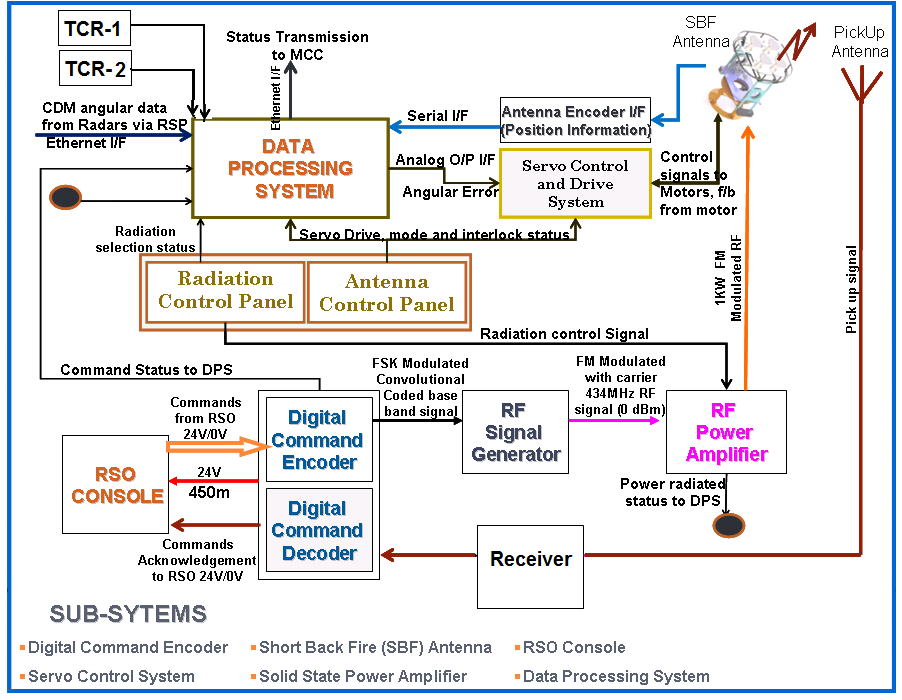
\includegraphics[width=\linewidth]{./Diagrams/TCSingleChainDiag.png}
	\caption{Single chain block diagram of Telecommand}
	\label{FIG:TcSingleChain}
\end{figure}

\begin{figure}[H]
	\centering
	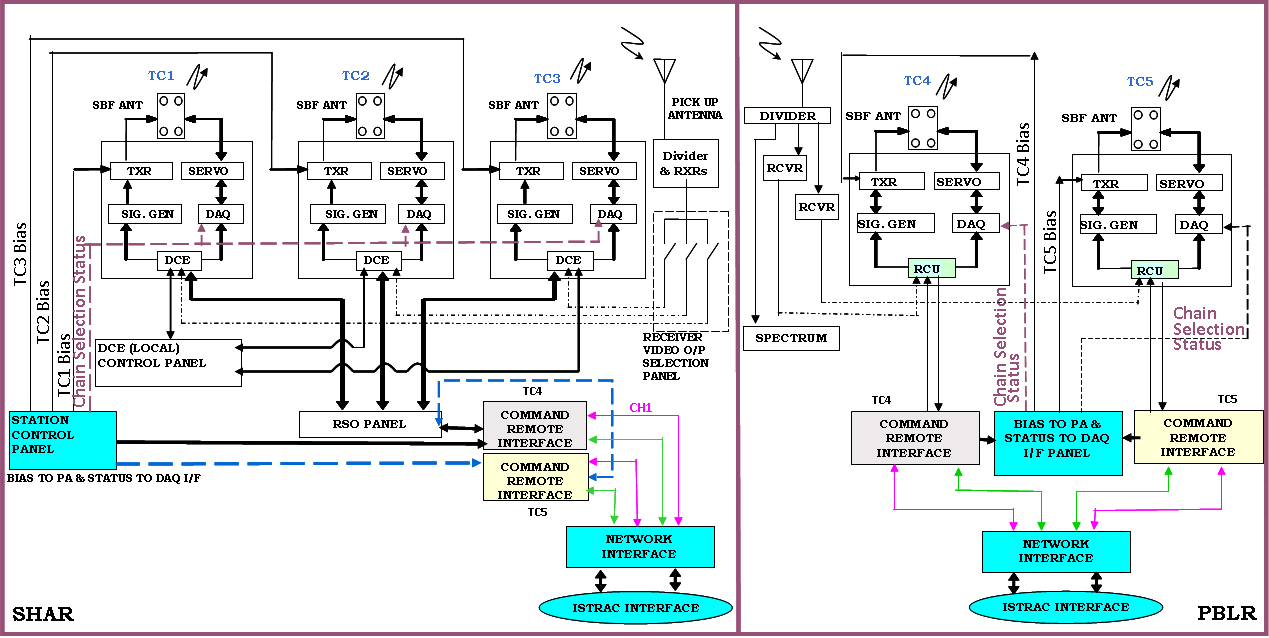
\includegraphics[width=\linewidth]{./Diagrams/TC5ChainConfg1.png}
	\caption{Five Chain Configuration of Telecommand}
	\label{FIG:FiveChConfig}
\end{figure}

\section{System Purpose}

\subsection{Data processing System}
Data Processing system is Intel Xeon 8 core processor CPU and application is designed in Qt Creator software tool on Linux platform. DPS generates error required for Azimuth and Elevation drive power amplifiers based on the present antenna positioned angle information and commanded angle information to keep the antenna orientation towards the vehicle trajectory. DPS acquires, processes, formats, packetises, displays and logs the data related to different sub-systems and the overall DPS schematic is shown in Fig. \ref{FIG:DPSSchematic}.

\begin{figure}[H]
	\centering
	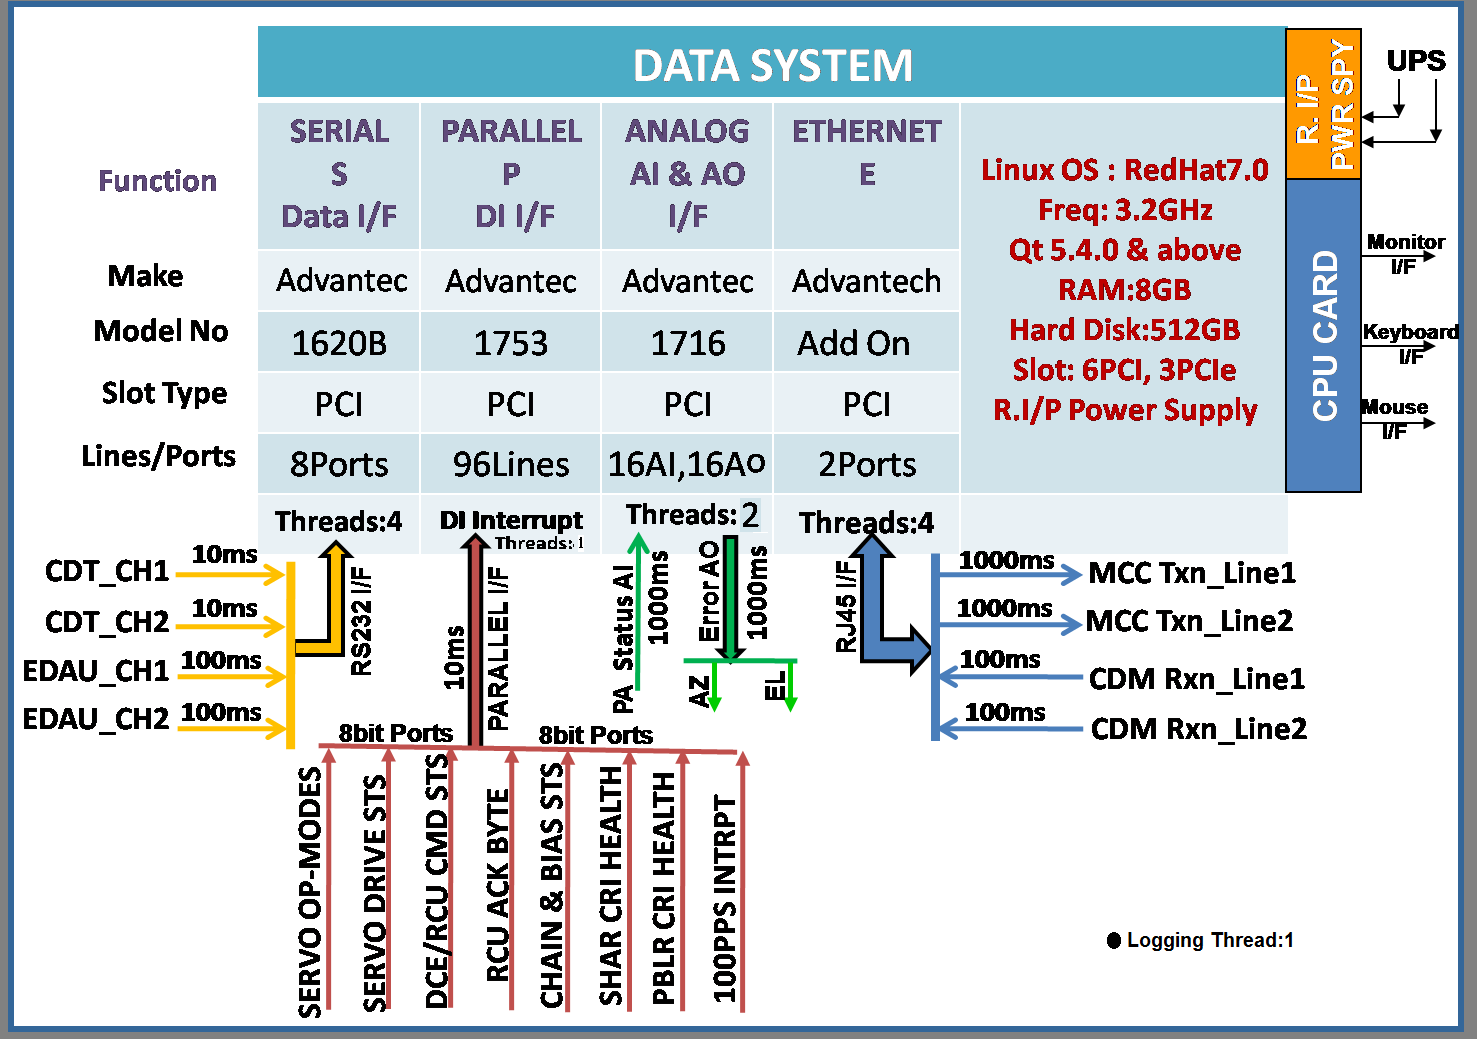
\includegraphics[width=\linewidth]{./Diagrams/DPSBlockDiagram.png}
	\caption{Overall Schematic of Data Processing System }
	\label{FIG:DPSSchematic}
\end{figure}


\subsection{Digital Command Encoder / Remote Command Unit }
Digital command encoder is based on convolution coding and decoder is based on Viterbi decoding which is implemented using FPGA board. The block level digram of DCE housed at SHAR TC is shown in Fig. \ref{FIG:DCEDiag}.The design of RCU unit positioned at PBLR is almost same as that of DCE except for the interfaces as shown in Fig. \ref{FIG:CRIConnectivity}. The system is capable of generating four commands SAFE, ARM, DESTRUCT, and COMMAND1 for vehicle command up-linking in real time.

\begin{figure}[H]
	\centering
	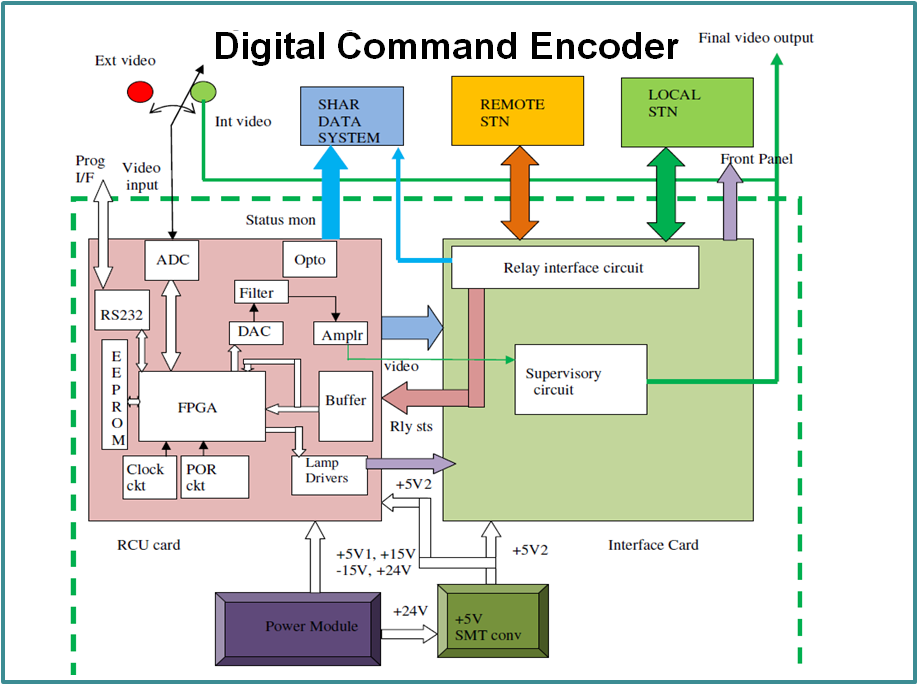
\includegraphics[width=\linewidth]{./Diagrams/DCEBlockDiag.png}
	\caption{Block Diagram of Digital Command Encoder }
	\label{FIG:DCEDiag}
\end{figure}

\subsection{Servo System}
Telecommand antenna movement is controlled using a servo system which consists of various sub systems like antenna driving motors, encoders, drive control modules, interlock logic system, operator control console, EDAU and DPS. Servo block diagram and its connectivity with other systems is shown in Fig. \ref{FIG:ServoDiag}. Antenna movement can be controlled either in open loop or closed loop. Open loop of operation includes applying joy stick deflection voltage to servo drive without involvement of DPS whereas closed loop systems includes either program mode or CDM mode for error generation using DPS and is fed to servo drive for steering the antenna.

\begin{figure}[H]
	\centering
	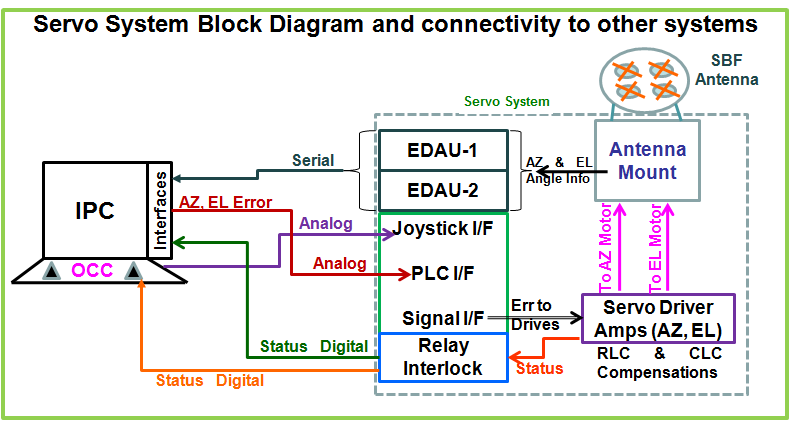
\includegraphics[width=\linewidth]{./Diagrams/BlockServo.png}
	\caption{Block Diagram of Servo System and connectivity to other systems }
	\label{FIG:ServoDiag}
\end{figure}


\subsection{Operator Control Console}
Antenna movement operations will be done from Operator Control Console. OCC consists of joysticks for manually controlling the antenna movement in open loop, operating switches and status indicators for various modes, drive power ON status, Emergency Stop operation and status indicators for pre-limit \& limit operation of antenna in both Azimuth \& Elevation axis. This is a part of servo system and is shown in Fig. \ref{FIG:ServoDiag}.

\subsection{Encoder Data Acquisition Unit}
EDAU is Microcontroller based system for acquiring, conversion from gray to binary format, converting to engineering units and displaying angular position of the antenna. It also transmits the angular information to DPS in serial format. EDAU is a part of servo systems is shown in Fig. \ref{FIG:ServoDiag}.

\subsection{Time Code Reader}
TCR provides timing information and interrupt for Telecommand DPS and 10 pps signal to EDAU unit for acquiring antenna encoder information. Single TCR provides timing information in two RS-232 ports, 10 pps \& 100 pps signals. Similar information from three TCRs is given to three TC chains at SHAR and from two TCRs is to two TC chains at PBLR in redundant cyclic manner as shown in Fig. \ref{FIG:SHARTIMINGDIST} and Fig. \ref{FIG:PBLRTIMINGDIST} respectively.

\begin{figure}[H]
	\centering
	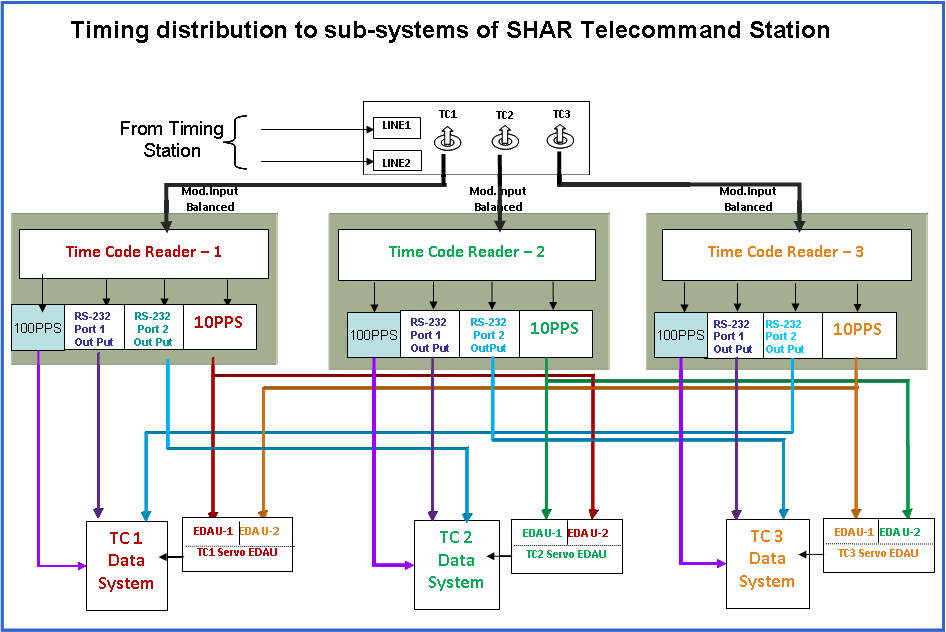
\includegraphics[width=0.9\linewidth]{./Diagrams/SharTimingDistribution.png}
	\caption{Timing distribution to sub-systems of Telecommand at SHAR}
	\label{FIG:SHARTIMINGDIST}
\end{figure}

\begin{figure}[H]
	\centering
	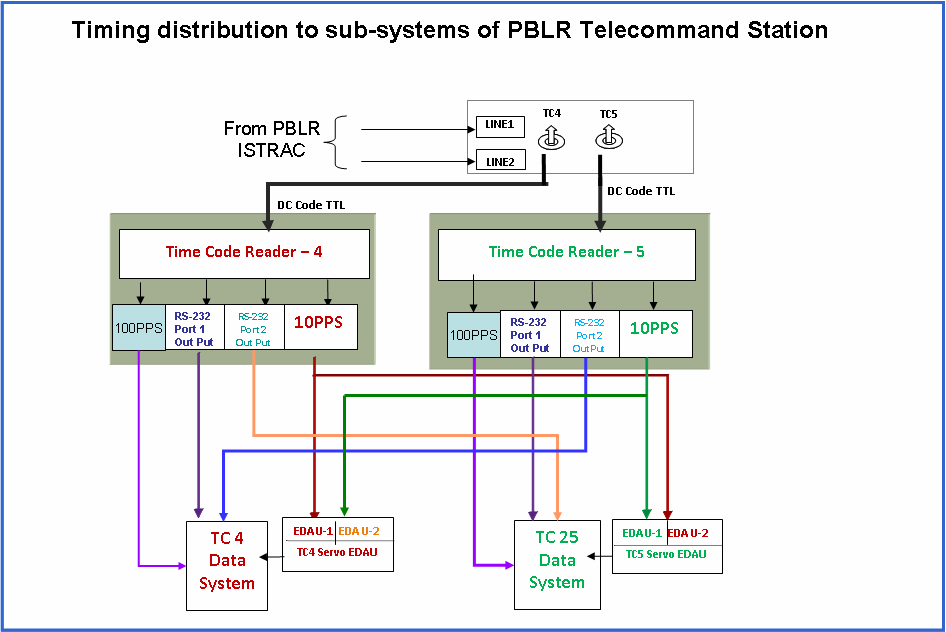
\includegraphics[width=0.9\linewidth]{./Diagrams/PBLRTimingDistribution.png}
	\caption{Timing distribution to sub-systems of Telecommand at PBLR}
	\label{FIG:PBLRTIMINGDIST}
\end{figure}


%\subsection{Integrated Telecommand Recorder}
%The command uplinked from antenna is received using a test antenna (spike/ quadra loop) and demodulated using receiver. The demodulated video output is fed back to DCE/RCU for decoding purpose. The same video output is logged using ITR at high rate (250KSps) so that actual command uplinked can be verified from logged data analysis.

\subsection{Transmitter/ Solid State Power Amplifier}
SSPA operates in the frequency band 400 to 500 MHz with a power output of 1 KW CW. Power amplifier is modular in construction, amplifies 0 dBm FM modulated RF signal to 60 dBm by employing different RF stages  and is shown in Fig. \ref{FIG:BlockPA}. ${V}_{f}$ is the DC calibrated power output and is interfaced to DPS via analog interface.

\begin{figure}[H]
	\centering
	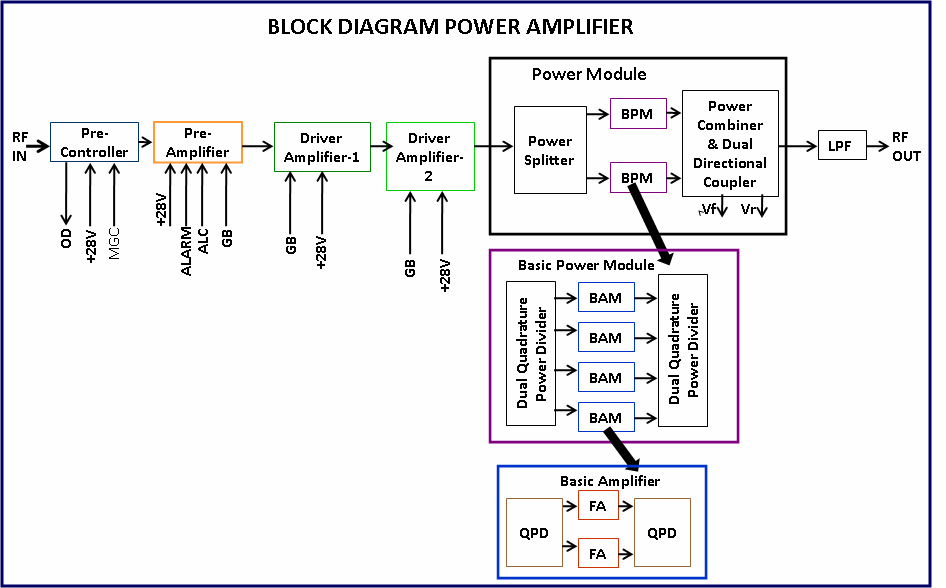
\includegraphics[width=\linewidth]{./Diagrams/BlockPA.png}
	\caption{Block Diagram of Power Amplifier}
	\label{FIG:BlockPA}
\end{figure}

\subsection{Short Back Fire Antenna}
Telecommand antenna is resonant, steerable wide beam antenna with elevation over azimuth mount. The antenna gain of 19 dBi and beam width of ${19}^{o}$ is achieved with four elements each with a gain of 13 dBi The antenna is an array of four elements each with a horizontal and vertical dipole. The antenna is called Short Back Fire antenna with RCP and the name is obtained based on its functionality. 

\subsection{Command Remote Interface}

The block level schematic of CRI showing the connectivity between RSO at SHAR with RCU at PBLR is shown in Fig. \ref{FIG:CRIConnectivity}. The CRI unit at SHAR end acquires command signal from RSO panel, Status \& control signals from SHAR TC control panel using PLC DI module.  Upon the detection of Command, the Processor will generate 2 words (2$\times$40=80 bits). Incase of SAFE or COMD1 the two words are same (Safe, Safe or comd1, comd1), whereas for DESTRUCT sequence the two words are ARM, DEST. Then these 80 bits along with source ID, bias status (radiation selection information), system in use status, CRC 16 bit polynomial check sum, packet counter, packet length are formed into 36 bytes packet and transmitted to PBLR via two ISTRAC links at 100 msec rate. \\ 

CRI at PBLR receives the packet at 100 msec rate. Change of command word will be sensed only if the three consecutive samples are same. Then, CRI transmits changed command word continuously at 100 msec rate using RS232 serial communication interface to RCU, otherwise CRI continues previous command word transmission to RCU at the same 100 msec rate. \\

CRI receives not only up-linked command status but also receives the residing command in RCU via serial RS232 interface. CRI in turn transmits the command uplinked status to RSO via ISTRAC links and command residing status to DPS via control panel.


\begin{figure}[H]
	\centering
	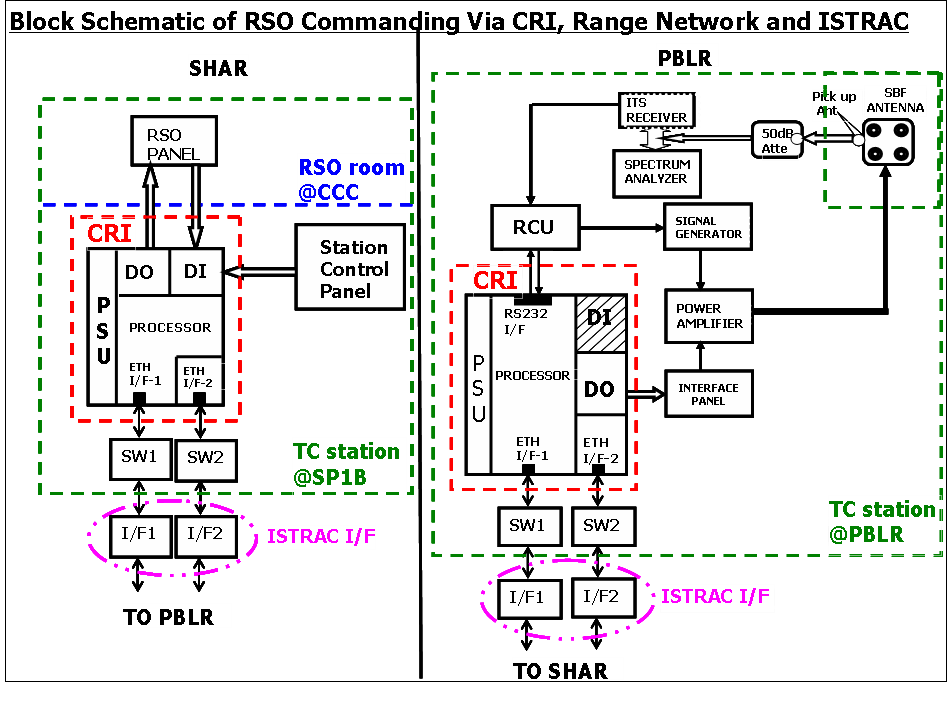
\includegraphics[width=\linewidth]{./Diagrams/BlockLevelSchematicCRISharPblr.png}
	\caption{Block level schematic of CRI connecting RSO at SHAR with RCU at PBLR}
	\label{FIG:CRIConnectivity}
\end{figure}

\section{System Scope}
The Software product named ``TC DPS" will be generated based on the Systems Requirements Specification document (SYRS) given in this document \cite{SYRSLBDPS}. Software Requirements Document (SRS) \cite{SRSLBDPS} will be generated based on SYRS and forms the base line document for software design. The industrial PC will be loaded with Red Hat Linux Enterprise version 7.0. The application will be developed in Qt Creator software tool in C++ programming language. The requirements of the TC DPS application software are mentioned in the following sections. This product does the following 

\begin{enumerate}
	\item [a)] Receives the antenna azimuth and elevation angles from the EDAU.
	\item [b)] Auto chain change over logic will be derived based on the healths of data received from EDAU chain-1 and chain-2.  
	\item [c)] Acquires the necessary inputs from the Telecommand subsystems like timing information from TCR; Status from DCE/RCU, Servo, CRI, Power Amplifier, Status Control Panel.
	\item [d)] Receives designated azimuth and elevation angles i.e., CDM data from RSP servers and processes them.
	\item [e)] Generates the necessary servo error voltages to drive the antenna so as to precisely point towards the launch vehicle in real time.
	\item [f)] The software will update the overall system status on the PC monitor display, provides Graphical User Interface (GUI).
	\item [g)] Logs the servo status, DCE parameters, EDAU parameters, station parameters, and incoming CDM data in the form of disk files.
	\item [h)] It also transmits station status parameters to MCC servers.
	
\end{enumerate}

The PCDPS, which is a part of the Telecommand system, is built around a Intel Xeon 8 core processor CPU card installed in an Industrial PC with a ${22}^{"}$ LED monitor, a keyboard, an optical mouse and redundant power supplies. The PC has a passive back plane with 6 PCI and 3 PCIe slots. These slots can accommodate the add-on cards required for the system to interact with all other subsystems of the Telecommand and the Real Time Network.